%% Overleaf			
%% Software Manual and Technical Document Template	
%% 									
%% This provides an example of a software manual created in Overleaf.

\documentclass{../ol-softwaremanual}

% Packages used in this example
\usepackage{graphicx}  % for including images
\usepackage{microtype} % for typographical enhancements
\usepackage{minted}    % for code listings
\usepackage{amsmath}   % for equations and mathematics
\setminted{style=friendly,fontsize=\small}
\renewcommand{\listoflistingscaption}{List of Code Listings}
\usepackage{hyperref}  % for hyperlinks
\usepackage[a4paper,top=4.2cm,bottom=4.2cm,left=3.5cm,right=3.5cm]{geometry} % for setting page size and margins

\usepackage[english, greek]{babel}

\usepackage{subfig}

\usepackage{incgraph,tikz}

\usepackage{filemod}
\usepackage{xcolor}




\usepackage{rotating}


% Custom macros used in this example document
\newcommand{\doclink}[2]{\href{#1}{#2}\footnote{\url{#1}}}
\newcommand{\cs}[1]{\texttt{\textbackslash #1}}

\begin{document}
	
	
	\begin{titlepage}
		
		
		% Frontmatter data; appears on title page
		\title{\en Use Cases \\}
		\version{0.2}
		\softwarelogo{
\includegraphics[scale=0.4]{../CarBazaar_logo.png}}		
		
	\end{titlepage}
	
	
	\maketitle
	
	\newpage
	
	\center{\textbf{Μέλη Ομάδας}}
	
	\vspace{20pt}
	
	
	
	\begin{table}[htbp!]
		
		\begin{tabular}{llll}
			Μεμελετζόγλου Χαρίλαος & 1069364 & \en st1069364@ceid.upatras.gr & 4o Έτος   \\ 
			\\ Λέκκας Γεώργιος      &      1067430    &   \en st1067430@ceid.upatras.gr & 4o Έτος  \\
			\\ Γιαννουλάκης Ανδρέας        &   1067387       & \en st1067387@ceid.upatras.gr & 4o Έτος           \\
			\\ Κανελλόπουλος Ιωακείμ        &  1070914        &    \en st1070914@ceid.upatras.gr & 4o Έτος        \\ 
		\end{tabular}
	\end{table}
	
	\center{\textbf{Υπεύθυνοι Παρόντος Τεχνικού Κειμένου}}
	
	\vspace{20pt}
	
	\begin{table}[htbp!]
		\begin{tabular}{ll}
			Μεμελετζόγλου Χαρίλαος & \en Editor \\
			\\ Λέκκας Γεώργιος      &   \en  Editor \\
			\\ Γιαννουλάκης Ανδρέας & \en Contributor \\
			\\ Κανελλόπουλος Ιωακείμ & \en Contributor \\ 
		\end{tabular}
	\end{table}


	\center{\textbf{Αλλαγές στην έκδοση \en v0.2 \gr}}
	\vspace{10pt}
	
	\begin{itemize}
		\item \en Use Case \textbf{1} \gr (\textit{Ανάρτηση Αγγελίας Πώλησης Οχήματος}) : Τροποποιήσεις και προσθήκες σε όλα τα βήματα της Βασικής Ροής (+ διαγραφές και συγχωνεύσεις κάποιων). Οι αλλαγές αυτές έγιναν με σκοπό την προσθήκη βημάτων όπως "εμφάνιση οθόνης" από το σύστημα, διεξαγωγή ελέγχων του συστήματος. Ακόμη, αλλαγές στην διατύπωση των βημάτων των Εναλλακτικών Ροών
		
		\item \en Use Case \textbf{2} \gr (\textit{Προγραμματισμός Ελέγχου Οχήματος}) : Τροποποιήσεις και προσθήκες σε όλα τα βήματα της Βασικής Ροής (+ διαγραφές και συγχωνεύσεις κάποιων). Σκοπός των αλλαγών αυτών ήταν η ρητή ανάδειξη της αλληλεπίδρασης χρήστη-συστήματος. Επίσης, προστέθηκε νέα Εναλλακτική Ροή \en \# \gr 2
		
		\item \en Use Case \textbf{5} \gr (\textit{Σύγκριση Αυτοκινήτων}) : Τροποποιήσεις σε βήματα της Βασικής Ροής, διαγραφές και συγχωνεύσεις κάποιων. Επέκταση του βήματος 1 της Εναλλακτικής Ροής \en \#\gr 1
		
		\item \en Use Case \textbf{7} \gr (\textit{Προγραμματισμός \en Test Drive\gr}) : Τροποποιήσεις σε βήματα της Βασικής Ροής, προσθήκες νέων (+ διαγραφές και συγχωνεύσεις κάποιων). Αλλαγή της διατύπωσης της Εναλλακτικής Ροής 1 + Προσθήκη Εναλλακτικής Ροής \en \#2\gr

		\item \en Use Case \textbf{12} \gr (\textit{Ανάρτηση Αγγελίας Πώλησης Ανταλλακτικού}) : Τροποποιήσεις σε βήματα της Βασικής Ροής, προσθήκες νέων (+ διαγραφές και συγχωνεύσεις κάποιων). Αλλαγή διατύπωσης των δύο Εναλλακτικών Ροών 
	\end{itemize}
	


	\newpage	
	
	\center{\textbf{Εργαλεία που χρησιμοποιήθηκαν}}
	
	\vspace{20pt}
	\flushleft
	Χρησιμοποιήθηκε το \en \doclink{https://www.overleaf.com/}{Overleaf} \gr και το \en \doclink{https://www.texstudio.org/}{TexStudio} \gr για την συγγραφή του \LaTeX\ κώδικα. \break
	
	Για την δημιουργία του λογότυπου, χρησιμοποιήθηκε το εργαλείο \en \doclink{https://www.adobe.com/express/create/logo}{Adobe Express} . \gr \break
	
	Για την δημιουργία του \en UML Use Case Diagram \gr χρησιμοποιήθηκε το \en \doclink{https://www.visual-paradigm.com/}{Visual Paradigm} . \gr \break 
	
	\newpage
	
	\center{\textbf{\en Use Cases \gr}}
	
	\paragraph{\en Use Case 1: \gr Ανάρτηση Αγγελίας Πώλησης Οχήματος}
	
	\begin{enumerate}
		
		\item Ο χρήστης επιλέγει \en"\gr Ανάρτηση Αγγελίας Οχήματος\en" \gr στο αρχικού μενού
		\item Το σύστημα εμφανίζει την οθόνη Καταχώρησης Αγγελίας Πώλησης Οχήματος
		\item Ο χρήστης εισάγει την τοποθεσία του, τον τίτλο της αγγελίας, στοιχεία του οχήματος όπως μάρκα, μοντέλο, έτος κυκλοφορίας, χιλιόμετρα, κυβικά, τύπος καυσίμου, χρώμα, αριθμός πινακίδας, κλπ
		\item Το σύστημα ελέγχει πως όντως κυκλοφορεί αντίστοιχο μοντέλο αυτοκινήτου στην αγορά και εμφανίζει στον χρήστη την Οθόνη Ανάρτησης Εγγράφων Πιστοποίησης Κατάστασης Οχήματος
		\item Ο χρήστης ανεβάζει τα απαραίτητα έγγραφα που έχουν προκύψει από τον έλεγχο του οχήματος		
		\item Το σύστημα εμφανίζει στον χρήστη μια εκτίμηση της τιμής του οχήματος, με βάση την κατάστασή του
		\item Ο χρήστης επιλέγει να συνεχίσει με την προτεινόμενη τιμή ή εισάγει δικιά του
		\item Το σύστημα μεταφέρει τον χρήστη στην οθόνη Εισαγωγής Φωτογραφιών και Περιγραφής Οχήματος
		\item Ο χρήστης προσθέτει το κείμενο της περιγραφής και αναρτά τις φωτογραφίες του αυτοκινήτου
		\item Το σύστημα δημιουργεί το \en 3D \gr μοντέλο του οχήματος και εμφανίζει μια προεπισκόπηση της αγγελίας στον χρήστη
		\item Ο χρήστης εγκρίνει την αγγελία
		\item Το σύστημα δημιουργεί την αγγελία και εμφανίζει μήνυμα επιτυχούς ανάρτησης
	\end{enumerate}
	
	\paragraph{Εναλλακτική Ροή 1}
	
	\begin{enumerate}
		\item O χρήστης εισάγει στοιχεία μη-υπαρκτού μοντέλου
		\item Το σύστημα εμφανίζει προειδοποιητικό μήνυμα, επιστρέφει τον χρήστη στην οθόνη \textit{Καταχώρηση Αγγελίας Οχήματος}, προτρέποντάς τον να διορθώσει τα λανθασμένα πεδία
		\item Ο χρήστης προβαίνει στις απαραίτητες διορθώσεις και η Περίπτωση Χρήσης συνεχίζει από το βήμα 4 της βασικής ροής
	\end{enumerate}
	
	\paragraph{Εναλλακτική Ροή 2}
	
	\begin{enumerate}
		\item Ο χρήστης δεν εισάγει περιγραφή ή δεν αναρτά φωτογραφίες του οχήματος
		\item Το σύστημα εμφανίζει προειδοποιητικό μήνυμα, επιστρέφει τον χρήστη στην οθόνη \textit{Εισαγωγή Φωτογραφιών και Περιγραφής Οχήματος}, προτρέποντάς τον, να συμπληρώσει τα αντίστοιχα πεδία
		\item Ο χρήστης εισάγει τις απαραίτητες ελλείπουσες πληροφορίες και η Περίπτωση Χρήσης συνεχίζει από το βήμα 9 της βασικής ροής
	\end{enumerate}
	
	\paragraph{Εναλλακτική Ροή 3}
	
	\begin{enumerate}
		\item Ο χρήστης εισάγει τιμή η οποία είναι σημαντικά μεγαλύτερη από την προτεινόμενη από το σύστημα, τιμή
		\item Το σύστημα εμφανίζει προειδοποιητικό μήνυμα, επιστρέφει τον χρήστη στον οθόνη \textit{Εισαγωγή Τιμής}, προτρέποντάς τον, να εισάγει τιμή που δεν αποκλίνει τόσο από την προτεινόμενη τιμή
		\item Ο χρήστης επανεισάγει τιμή και η Περίπτωση Χρήσης συνεχίζει από το βήμα 8 της βασικής ροής
	\end{enumerate}
	
	
	\paragraph{\en Use Case 2: \gr Προγραμματισμός Ελέγχου Οχήματος}
	
	\begin{enumerate}
		\item Ο χρήστης επιλέγει \en"\gr Έλεγχος Οχήματος\en" \gr στο αρχικό μενού
		\item Το σύστημα εμφανίζει την σελίδα Προγραμματισμού Ελέγχου Οχήματος
		\item Ο χρήστης επιλέγει το πακέτο ελέγχου που επιθυμεί, αν επιθυμεί την έκδοση πιστοποιητικών εγγράφων της κατάστασης του οχήματος, την ημερομηνία και ώρα διεξαγωγής του ελέγχου και εισάγει την τοποθεσία του
		\item Το σύστημα αφού επιβεβαιώσει την εισαχθείσα τοποθεσία, προτείνει στην χρήστη έναν ελεγκτή, με βάση την τοποθεσία που εισήγαγε
		\item Ο χρήστης αποδέχεται ή όχι τον προτεινόμενο ελεγκτή
		\item Το σύστημα εμφανίζει την οθόνη Εισαγωγή Κωδικού Αγγελίας, στο όχημα της οποίας θα πραγματοποιηθεί ο έλεγχος		
		\item Ο χρήστης εισάγει τον κωδικό της αγγελίας
		\item Το σύστημα ανακτά τα στοιχεία του οχήματος από την αγγελία και εμφανίζει την τελική τιμή του ελέγχου καθώς και την χρονική διάρκειά του
		\item Ο χρήστης επιβεβαιώνει τα στοιχεία
		\item Το σύστημα μεταφέρει τον χρήστη στο μενού πληρωμών. Μετά την επιτυχή πληρωμή, εμφανίζει μήνυμα επιτυχούς κράτησης και αποστέλλει \en email \gr στον χρήστη, με τα στοιχεία του ραντεβού και του ελεγκτή		
	\end{enumerate}
	
	\paragraph{Εναλλακτική Ροή 1}
	
	\begin{enumerate}
		\item Ο χρήστης εισάγει μη-υπαρκτή τοποθεσία
		\item Το σύστημα ενημερώνει τον χρήστη με το κατάλληλο μήνυμα σφάλματος 
		\item Ο χρήστης εισάγει την σωστή τοποθεσία του
		\item Το σύστημα εντοπίζει τον χρήστη και η Περίπτωση Χρήσης προχωρά από το βήμα 4 της βασικής ροής
	\end{enumerate}

	\paragraph{\red{Εναλλακτική Ροή 2}}
	
\red {\begin{enumerate}
		\item Ο χρήστης απορρίπτει τον προτεινόμενο από το σύστημα ελεγκτή, προκειμένου να επιλέξει τον ελεγκτή της αρεσκείας του
		\item Το σύστημα εμφανίζει την οθόνη εισαγωγής στοιχείων του ελεγκτή
		\item Ο χρήστης εισάγει τα στοιχεία του ελεγκτή
		\item Το σύστημα ελέγχει πως υπάρχει πράγματι εγγεγραμμένος ο εν λόγω ελεγκτής και αν ναι, η Περίπτωση Χρήσης συνεχίζει από το βήμα 6 της βασικής ροής. Ειδάλλως, εμφανίζει μήνυμα σφάλματος και ο έλεγχος ακυρώνεται	
	\end{enumerate}	}
	
	
	
	\paragraph{\en Use Case 3: \gr Αναζήτηση Ανταλλακτικού}	
	
	\begin{enumerate}
		\item Ο χρήστης επιλέγει στο μενού της εφαρμογής την κατηγορία  \en"\gr Ανταλλακτικά \en"\gr
		\item Το σύστημα εμφανίζει στον χρήστη μια οθόνη με πολλαπλά πεδία και φίλτρα
		\item Ο χρήστης περιορίζει την αναζήτηση του τοποθετώντας το είδος του οχήματος,την μάρκα,το μοντέλο,τον κατασκευαστή,το εύρος τιμών, και την κατάσταση του ανταλλακτικού(καινούργιο ή μεταχειρισμένο) 
		\item Το σύστημα εμφανίζει τη λίστα με τις αγγελίες που πληρούν τα κριτήρια που έθεσε ο χρήστης
		\item Ο χρήστης επιλέγει την αγγελία της αρεσκείας του
		\item Το σύστημα εμφανίζει μια λεπτομερή περιγραφή του ανταλλακτικού και τα στοιχεία του πωλητή
		
	\end{enumerate}
	
	\paragraph{Εναλλακτική Ροή}
	
	\begin{enumerate}
		\item Ο χρήστης δεν εισάγει χαρακτηριστικά για το ανταλλακτικό που επιθυμεί να αγοράσει
		\item Το σύστημα του εμφανίζει ανταλλακτικά για όλες τις κατηγορίες και μάρκες αυτοκινήτων και προχωρά από το βήμα 4 της βασικής ροής
	\end{enumerate}
	
	\paragraph{\en Use Case 4: \gr Αναζήτηση Κοντινών Αντιπροσωπειών}	
	
	\begin{enumerate}
		\item Ο χρήστης επιλέγει στο μενού της εφαρμογής την κατηγορία \en"\gr Εύρεση Κοντινών Αντιπροσωπειών \en"\gr
		\item Το σύστημα εμφανίζει ένα χάρτη και ένα πεδίο αναζήτησης, προτρέποντας τον χρήστη να εισάγει την περιοχή του
		\item Ο χρήστης εισάγει την περιοχή του  
		\item Το σύστημα εμφανίζει όλες τις αντιπροσωπείες που βρίσκονται κοντα στην περιοχή που έθεσε ο χρήστης
		\item Ο χρήστης επιλέγει την αντιπροσωπεία της αρεσκείας του
		\item Το σύστημα εμφανίζει μία λίστα με οχήματα που είναι διαθέσιμα από την αντιπροσωπεία     	
	\end{enumerate}
	
	
	
	\paragraph{\en Use Case 5: \gr Σύγκριση Αυτοκινήτων}
	\begin{enumerate}
		\item Ο χρήστης επιλέγει \en"\gr Σύγκριση Αυτοκινήτων\en" \gr στο αρχικό μενού
		\item Το σύστημα εμφανίζει την οθόνη Σύγκρισης Αυτοκινήτων και προτρέπει τον χρήστη να εισάγει τους κωδικούς διαφορετικών αγγελιών, τα οχήματα των οποίων επιθυμεί να συγκρίνει
		\item Ο χρήστης εισάγει τους κωδικούς των αγγελιών
		\item Το σύστημα ελέγχει αν εισήχθησαν κωδικοί και αν είναι διαφορετικοί μεταξύ τους. Στην συνέχεια, εμφανίζει την οθόνη Κριτήρια Αυτοκινήτων προς Σύγκριση, προτρέποντας τον χρήστη να εισάγει το επιθυμητό εύρος τιμών και τα σημαντικά κριτήρια που θα συντελέσουν στην επιλογή ενός οχήματος
		\item Ο χρήστης εισάγει το επιθυμητό εύρος τιμών και καθορίζει τα κυρίαρχα κριτήρια της σύγκρισης
		\item Το σύστημα εμφανίζει την οθόνη Αποτελέσματα Αναζήτησης, προβάλλοντας μία λίστα με τα αυτοκίνητα και τα χαρακτηριστικά που ο χρήστης επέλεξε να πάρουν μέρος στην σύγκριση, αλλά και το κόστος των τελών κυκλοφορίας και των ασφαλίστρων. Επίσης, το σύστημα προτείνει στον χρήστη κατάλληλα οχήματα με βάση τα κριτήρια σύγκρισης
		\item Ο χρήστης επιλέγει το όχημα που επιθυμεί
		\item Το σύστημα μεταφέρει τον χρήστη στην οθόνη Λεπτομέρειες Αγγελίας, επιτρέποντάς του να εξετάσει αναλυτικότερα το επιλεγμένο όχημα
	\end{enumerate}
	
	\paragraph{Εναλλακτική Ροή 1}
	
	\begin{enumerate}
		\item Ο χρήστης δεν εισάγει κωδικούς αγγελιών \red{ή οι κωδικοί που εισήγαγε δεν είναι διαφορετικοί μεταξύ τους}
		\item Το σύστημα εμφανίζει προειδοποιητικό μήνυμα και προτείνει στον χρήστη παρόμοια οχήματα με αυτά που έχει αποθηκεύσει στην \en wishlist \gr του αλλά και οχήματα που συμμετέχουν συχνά σε συγκρίσεις άλλων χρηστών
		\item Ο χρήστης καθορίζει τα κριτήρια σύγκρισης και η Περίπτωση Χρήσης συνεχίζει από το βήμα 5 της βασικής ροής
	\end{enumerate}
	
	
	\paragraph{\en Use Case 6: \gr Προσθήκη Καταστήματος Αντιπροσωπείας}
	
	\begin{enumerate}
		\item Ο υπεύθυνος της αντιπροσωπείας επιλέγει \en"\gr Προσθήκη Καταστήματος \en"\gr
		\item Το σύστημα ζητά από τον χρήστη το όνομα της εταιρείας στην οποία υπάγεται η αντιπροσωπεία
		\item Ο υπεύθυνος εισάγει το όνομα της εταιρείας
		\item Το σύστημα επιβεβαιώνει πως στην Βάση Δεδομένων της πλατφόρμας, υπάρχει εγγεγραμμένη η αντίστοιχη εταιρεία		
		\item Το σύστημα εμφανίζει τον χάρτη και ζητά από τον χρήστη να εισάγει την τοποθεσία του καταστήματος
		\item Ο υπεύθυνος της αντιπροσωπείας εισάγει τα λεπτομερή γεωγραφικά στοιχεία του καταστήματος
		\item Το σύστημα εντοπίζει το κατάστημα στον χάρτη και ζητά επιβεβαίωση από τον χρήστη
		\item Ο υπεύθυνος επιβεβαιώνει την ορθότητα των στοιχείων		
		\item Το σύστημα ζητά από τον χρήστη να εισάγει τον τίτλο του καταστήματος και μια λίστα με τα αυτοκίνητα που διαθέτει προς πώληση
		\item Ο υπεύθυνος εισάγει τον τίτλο και τα οχήματα που διαθέτει το κατάστημα
		\item Το σύστημα ρωτάει τον χρήστη αν επιθυμεί να δημιουργήσει μια διαφήμιση για το συγκεκριμένο κατάστημα, με σκοπό την ενημέρωση των χρηστών της πλατφόρμας που βρίσκονται στην περιοχή του καταστήματος
		\item Ο υπεύθυνος επιλέγει την δημιουργία της σχετικής διαφήμισης
		\item Το σύστημα ανακατευθύνει τον χρήστη στο παράθυρο δημιουργίας διαφήμισης			
	\end{enumerate}
	
	\paragraph{Εναλλακτική Ροή 1}
	
	\begin{enumerate}
		\item Ο υπεύθυνος της αντιπροσωπείας εισάγει όνομα εταιρείας, η οποία δεν ανήκει στην πλατφόρμα
		\item Το σύστημα ενημερώνει τον χρήστη σχετικά με το σφάλμα και τον ρωτά αν επιθυμεί να εγγράψει στην πλατφόρμα, την εταιρεία με το όνομα που εισήγαγε
		\item Ο υπεύθυνος επιλέγει εγγραφή 
		\item Το σύστημα ανακατευθύνει τον χρήστη στο μενού εγγραφής εταιρείας
	\end{enumerate}
	
	\paragraph{\en Use Case 7: \gr Προγραμματισμός \en Test Drive \gr}
	
	\begin{enumerate}
		\item Ο χρήστης επιλέγει \en"Test Drive" \gr στο αρχικό μενού
		\item Το σύστημα εμφανίζει την οθόνη οθόνη Καταχώρησης Κωδικού Αγγελίας Οχήματος
		\item Ο χρήστης εισάγει τον κωδικό της αγγελίας, για το όχημα της οποίας ενδιαφέρεται για \en Test Drive \gr
		\item Το σύστημα ελέγχει πως ο κωδικός αντιστοιχεί σε καταχωρημένη αγγελία και μεταφέρει τον χρήστη στην οθόνη Προγραμματισμού \en Test Drive \gr
		\item Ο χρήστης εισάγει την επιθυμητή ημερομηνία και ώρα
		\item Το σύστημα εμφανίζει τα στοιχεία του ραντεβού
		\item Ο χρήστης επιβεβαιώνει τα στοιχεία
		\item Το σύστημα εμφανίζει την οθόνη Επιτυχούς προγραμματισμού \en Test Drive \gr και αποστέλλει στο \en email \gr του χρήστη και του πωλητή του οχήματος, τα λεπτομερή στοιχεία του ραντεβού 
	\end{enumerate}
	
	\paragraph{Εναλλακτική Ροή 1}
	
	\begin{enumerate}
		\item Ο χρήστης επιλέγει μη-διαθέσιμη ημερομηνία και ώρα
		\item Το σύστημα εμφανίζει μήνυμα σφάλματος σχετικά με την μη-διαθεσιμότητα της επιλεγμένης ημερομηνίας και μεταφέρει τον χρήστη στην οθόνη \textit{Προγραμματισμού \en Test Drive \gr}, προτρέποντάς τον επιλέξει ξανά
		\item Ο χρήστης επιλέγει νέα ημερομηνία και ώρα και η Περίπτωση Χρήσης συνεχίζει από το βήμα 6 της βασικής ροής
	\end{enumerate}


	\paragraph{\red{Εναλλακτική Ροή 2}}
	
	\red{\begin{enumerate}
		\item Ο χρήστης εισάγει κωδικό μη-καταχωρημένης αγγελίας
		\item Το σύστημα εμφανίζει σχετικό μήνυμα σφάλματος και μεταφέρει τον χρήστη στην οθόνη \textit{Καταχώρησης Κωδικού Αγγελίας Οχήματος}, προτρέποντάς τον να επανεισάγει τον κωδικό
		\item Ο χρήστης εισάγει τον κωδικό της αγγελίας και η Περίπτωση Χρήσης συνεχίζει από το βήμα 4 της βασικής ροής
	\end{enumerate}}
	
	
	\paragraph{\en Use Case 8: \gr  Ανταλλαγή Οχημάτων \gr}
	
	\begin{enumerate}
		\item Ο χρήστης επιλέγει \en"\gr Ανταλλαγή Οχήματος \en"\gr 
		\item Το σύστημα ζητά από τον χρήστη να εισάγει τον κωδικό της αγγελίας του οχήματος που επιθυμεί να ανταλλάξει και τον κωδικό της αγγελίας του οχήματος που επιθυμεί να αποκτήσει 
		\item Ο χρήστης εισάγει τους κωδικούς των δύο αγγελιών 	
		\item Το σύστημα αποστέλλει \en email \gr στον πωλητή του οχήματος της αγγελίας, προκειμένου να τον ενημερώσει για το αίτημα ανταλλαγής
		\item Ο χρήστης αποστέλλει μήνυμα στον πωλητή, προκειμένου να διευθετηθούν τα απαραίτητα διαδικαστικά ζητήματα 
		\item Οι δύο χρήστες ανεβάζουν στην πλατφόρμα τα απαραίτητα νομικά έγγραφα για την μεταβίβαση των οχημάτων και η ανταλλαγή ολοκληρώνεται
	\end{enumerate}
	
	\paragraph{Εναλλακτική Ροή 1}
	
	\begin{enumerate}
		\item Ο χρήστης εισάγει κωδικό αγγελίας που δεν αντιστοιχεί σε αγγελία που έχει καταχωρήσει
		\item Το σύστημα προτρέπει τον χρήστη να δημιουργήσει μια \en"\gr Προσωρινή Αγγελία\en"\gr, προκειμένου να προχωρήσει η διαδικασία της ανταλλαγής
		\item Ο χρήστης εισάγει χαρακτηριστικά του οχήματος, όπως την μάρκα, το μοντέλο, την κατάσταση του οχήματος, τα χιλιόμετρα και τυχόν μηχανικά προβλήματα, μια σύντομη περιγραφή καθώς και φωτογραφίες του οχήματος
		\item Το σύστημα εμφανίζει στον χρήστη μια εκτίμηση της τιμής του οχήματος
		\item Ο χρήστης αποδέχεται την προτεινόμενη τιμή ή εισάγει μια δικιά του, και η Περίπτωση Χρήσης συνεχίζει από το βήμα 4 της βασικής ροής
		
	\end{enumerate}       
	
	
	\paragraph{Εναλλακτική Ροή 2}
	\begin{enumerate}
		\item Ο χρήστης επιθυμεί να ανταλλάξει όχημα του οποίου είτε η προτεινόμενη είτε η καθορισμένη από τον χρήστη τιμή, διαφέρει σημαντικά από την τιμή του οχήματος που επιθυμεί να αποκτήσει
		\item Το σύστημα εμφανίζει το αντίστοιχο μήνυμα σφάλματος και προχωρά στην ακύρωση της ανταλλαγής 
	\end{enumerate}
	
	\paragraph{\en Use Case 9: \gr Αγορά Οχήματος\gr}
	
	\begin{enumerate}
		\item Ο χρήστης επιλέγει \en"\gr Αγορά Οχήματος \en"\gr
		\item Το σύστημα αποστέλλει έναν κωδικό ασφαλείας στο \en email \gr του χρήστη
		\item Ο χρήστης εισάγει τον κωδικό ασφαλείας		
		\item Το σύστημα ζητά από τον χρήστη τον κωδικό της αγγελίας του οχήματος που επιθυμεί να αγοράσει
		\item Ο χρήστης εισάγει τον κωδικό της αγγελίας	
		\item To σύστημα ρωτά τον χρήστη αν επιθυμεί να πληρώσει με άτοκες δόσεις
		\item Ο χρήστης αποκρίνεται καταφατικά			
		\item Το σύστημα ρωτά τον χρήστη αν επιθυμεί να χρησιμοποιήσει την υπηρεσία \en"\gr Οικονομικός Σύμβουλος \en"\gr.
		\item Ο χρήστης επιλέγει να χρησιμοποιήσει την υπηρεσία προκειμένου να διαπιστώσει αν μπορεί να αντεπεξέλθει στα έξοδα 
		\item Το σύστημα ζητά από τον χρήστη να εισάγει τον μηνιαίο μισθό του, με σκοπό τον υπολογισμό ενός προσαρμοσμένου στον χρήστη, ποσού άτοκης μηνιαίας δόσης
		\item Το σύστημα εμφανίζει το υπολογισμένο ποσό καθώς και το κόστος των τελών κυκλοφορίας του οχήματος
		\item Ο χρήστης αποδέχεται το ποσό της μηνιαίας δόσης
		\item Το σύστημα εμφανίζει την συνολική τιμή καθώς και τον κωδικό της αγγελίας και το όνομα του οχήματος και μεταφέρει τον χρήστη στην σελίδα του συστήματος πληρωμών
		\item Ο χρήστης πληρώνει για την αγορά του οχήματος
		\item Το σύστημα εμφανίζει μήνυμα επιτυχούς αγοράς και αποστέλλει στο \en email \gr του χρήστη την απόδειξη πληρωμής καθώς και τον κωδικό της συναλλαγής
	\end{enumerate}
	
	\paragraph{Εναλλακτική Ροή 1}
	\begin{enumerate}
		\item Ο χρήστης επιλέγει να μην πληρώσει με άτοκες δόσεις και η Περίπτωση Χρήσης συνεχίζει από το βήμα 13 της βασικής ροής
	\end{enumerate}
	
	\paragraph{Εναλλακτική Ροή 2}
	\begin{enumerate}
		\item Ο χρήστης εισάγει κωδικό μη-υπαρκτής αγγελίας
		\item Το σύστημα ενημερώνει τον χρήστη
		\item Ο χρήστης διορθώνει τον κωδικό και η Περίπτωση Χρήσης συνεχίζει από το βήμα 6 της βασικής ροής
	\end{enumerate}
	
	\paragraph{\en Use Case 10: \gr Αναζήτηση Οχήματος}  
	\begin{enumerate}
		\item Ο χρήστης επιλέγει το πεδίο \en"\gr Αναζήτηση Οχήματος \en"\gr
		\item Το σύστημα προτρέπει τον χρήστη να εισάγει τα χαρακτηριστικά του οχήματος ή να εισάγει το όνομά του, καθώς και το εύρος τιμών εντός του οποίου πρέπει να βρίσκονται τα αποτελέσματα
		\item Ο χρήστης συμπληρώνει όσα πεδία επιθυμεί ή εκτελεί αναζήτηση με βάση το όνομα του οχήματος
		\item Το σύστημα ρωτά τον χρήστη αν επιθυμεί να εμφανιστούν αγγελίες από ιδιώτες χρήστες ή/και από αντιπροσωπείες, το κριτήριο ταξινόμησης των αγγελιών καθώς και να εισάγει την τοποθεσία του και την ακτίνα αναζήτησης		
		\item Το σύστημα εμφανίζει την λίστα με τις αγγελίες που πληρούν τα κριτήρια που έθεσε ο χρήστης	
		\item Ο χρήστης επιλέγει μια αγγελία με σκοπό να δει λεπτομέρειες για το όχημα
		\item Το σύστημα εμφανίζει την περιγραφή της αγγελίας, τα χαρακτηριστικά του οχήματος, μια \en 3D \gr απεικόνιση του οχήματος, τα στοιχεία επικοινωνίας του πωλητή καθώς και κριτικές που πιθανόν να έχει λάβει		
	\end{enumerate}
	
	\paragraph{Εναλλακτική Ροή 1}
	\begin{enumerate}
		\item  Ο χρήστης εκτελεί αναζήτηση με βάση το όνομα και εισάγει όνομα που δεν αντιστοιχεί σε υπαρκτό όχημα
		\item Το σύστημα ενημερώνει τον χρήστη και του ζητά να διορθώσει το όνομα
		\item Ο χρήστης εισάγει το σωστό όνομα και η Περίπτωση Χρήση συνεχίζει από το βήμα 4 της βασικής ροής		 
	\end{enumerate}
	
	\paragraph{Εναλλακτική Ροή 2}
	\begin{enumerate}
		\item Ο χρήστης εισάγει μη-υπαρκτή τοποθεσία
		\item Το σύστημα ενημερώνει το χρήστη και τον προτρέπει να εισάγει νέα τοποθεσία 
		\item Ο χρήστης εισάγει νέα τοποθεσία και η Περίπτωση Χρήσης συνεχίζει από το βήμα 5 της βασικής ροής
	\end{enumerate}
	
	
	
	
	\paragraph{\en Use Case 11: \gr Επεξεργασία Αγγελίας \gr}
	
	\begin{enumerate}
		\item Ο χρήστης επιλέγει \en"\gr Οι αγγελίες μου \en"\gr
		\item Το σύστημα εμφανίζει μια λίστα με όλες τις αγγελίες που έχει αναρτήσει, με στοιχεία όπως ημερομηνία καταχώρισης, κατάσταση (αν έχει πουληθεί το προϊόν ή όχι), αριθμός προβολών αγγελίας
		\item Ο χρήστης επιλέγει την αγγελία που επιθυμεί να επεξεργαστεί
		\item Το σύστημα εμφανίζει στον χρήστη ένα μενού με επιλογές, όπως \en"\gr Επεξεργασία Περιγραφής \en"\gr , \en"\gr Επεξεργασία Φωτογραφιών \en"\gr,\en"\gr Επεξεργασία Χαρακτηριστικών Οχήματος/Ανταλλακτικού \en"\gr, \en"\gr Επεξεργασία Τιμής \en"\gr
		\item Ο χρήστης επιλέγει την επιλογή που επιθυμεί και προχωρά στις επιθυμητές αλλαγές
		\item Το σύστημα εμφανίζει μια προεπισκόπηση της νέα μορφής της αγγελίας
		\item Ο χρήστης αποδέχεται τις αλλαγές
	\end{enumerate}
	
	\paragraph{\en Use Case 12: \gr Ανάρτηση Αγγελίας Πώλησης Ανταλλακτικού \gr}
	
	\begin{enumerate}
		\item Ο χρήστης επιλέγει \en"\gr Ανάρτηση Αγγελίας Ανταλλακτικού \en"\gr στο αρχικό μενού
		\item Το σύστημα εμφανίζει την οθόνη Ανάρτησης Αγγελίας Ανταλλακτικού
		\item Ο χρήστης εισάγει την τοποθεσία του και τον τίτλο της αγγελίας
		\item Το σύστημα εμφανίζει την οθόνη Εισαγωγή στοιχείων Ανταλλακτικού
		\item Ο χρήστης εισάγει στοιχεία του ανταλλακτικού όπως η κατάστασή του (καινούριο ή μεταχειρισμένο), τον τύπο του, τον κωδικό του, την εταιρεία, το μοντέλο και την τιμή του
		\item Το σύστημα ελέγχει πως όντως υπάρχει ανταλλακτικό με τον δοσμένο κωδικό, εμφανίζει την οθόνη Κατηγορίες Ανταλλακτικών, και προτρέπει τον χρήστη να εισάγει την περιγραφή του ανταλλακτικού αλλά και φωτογραφίες του
		\item Ο χρήστης εισάγει περιγραφή και αναρτά τις απαραίτητες φωτογραφίες
		\item Το σύστημα εμφανίζει την οθόνη Εισαγωγή Δωρεάν Ανταλλακτικού, προτρέποντας τον χρήστη να προσφέρει κάποιο ανταλλακτικό χαμηλότερης αξίας ως δώρο μαζί με το κύριο ανταλλακτικό, με σκοπό την ταξινόμηση της αγγελίας του υψηλότερα στα αποτελέσματα αναζήτησης
		\item Ο χρήστης εισάγει τα χαρακτηριστικά και την τιμή του δωρεάν ανταλλακτικού
		\item Το σύστημα εμφανίζει δημιουργεί την αγγελία, καταχωρεί το κύριο ανταλλακτικό στην κατάλληλη κατηγορία με βάση τον κωδικό του και εμφανίζει μια προεπισκόπηση της αγγελίας
		\item Ο χρήστης εγκρίνει την αγγελία
		\item Το σύστημα δημιουργεί την αγγελία και εμφανίζει μήνυμα επιτυχούς ανάρτησης
	\end{enumerate}


	\paragraph{Εναλλακτική Ροή 1}
	
	\begin{enumerate}
		\item Ο χρήστης εισάγει κωδικό μη-υπαρκτού ανταλλακτικού
		\item Το σύστημα εμφανίζει προειδοποιητικό μήνυμα και επιστρέφει τον χρήστη στην Οθόνη \textit{Εισαγωγή στοιχείων Ανταλλακτικού}
		\item Ο χρήστης επανεισάγει τον κωδικό και η Περίπτωση Χρήσης προχωρά από το βήμα 4 της βασικής ροής
	\end{enumerate}
	
	\paragraph{Εναλλακτική Ροή 2}
	
	\begin{enumerate}
		\item Ο χρήστης εισάγει ως δωρεάν ανταλλακτικό, παραπλήσιας αξίας με το κύριο ανταλλακτικό της αγγελίας
		\item Το σύστημα εμφανίζει μήνυμα προειδοποίησης, ενημερώνοντάς τον χρήστη πως το δεύτερο ανταλλακτικό δεν είναι αρκετά φθηνότερο από το κύριο ανταλλακτικό ώστε να προσφερθεί ως δώρο και επιστρέφει τον χρήστη στην οθόνη \textit{Εισαγωγή Δωρεάν Ανταλλακτικού}
		\item Ο χρήστης είτε εισάγει διαφορετικό δωρεάν ανταλλακτικό, είτε προχωρά χωρίς δωρεάν ανταλλακτικό και η Περίπτωση Χρήσης προχωρά από το βήμα 10 της βασικής ροής
	\end{enumerate}
	
	
	\paragraph{\en Use Case 13: \gr Έλεγχος Αναφοράς}  
	\begin{enumerate}
		\item Ο υπάλληλος της Ασφαλιστικής εταιρείας επιλέγει το πεδίο \en"\gr Έλεγχος αναφοράς\en"\gr
		\item Το σύστημα εμφανίζει την λίστα με τις αναφορές, τον κωδικό τους και την κατάστασή τους (\en"\gr σε εκκρεμότητα \en" \gr κλπ)
		\item Ο υπάλληλος επιλέγει ή εισάγει τον κωδικό της αναφοράς που επιθυμεί να ελέγξει 
		\item Το σύστημα εμφανίζει την αγγελία και την λίστα με τις αναφορές που έχει λάβει, καθώς και στοιχεία αυτών όπως τον δημιουργό, την ημερομηνία υποβολής και την αιτία αναφοράς 
		\item Ο υπάλληλος της εταιρείας, εξετάζει την αγγελία και αν η αναφορά είναι βάσιμη, προχωρά στην διαγραφή της αγγελίας ενημερώνοντας και τον δημιουργό της αναφοράς αλλά και τον δημιουργό της αγγελίας. Ειδάλλως, σε περίπτωση ψευδούς αναφοράς, η αναφορά σημειώνεται ως ψευδής και ο έλεγχος ολοκληρώνεται
	\end{enumerate}
	
	\paragraph{Εναλλακτική Ροή 1}
	\begin{enumerate}
		\item Ο υπάλληλος της ασφαλιστικής εταιρείας εισάγει κωδικό αναφοράς που δεν αντιστοιχεί σε κάποια υπάρχουσα
		\item Το σύστημα ενημερώνει τον υπάλληλο  για το λάθος και τον προτρέπει  να εισάγει ορθό κωδικό 
		\item Ο υπάλληλος εισάγει τον κωδικό αναφοράς ξανά
		\item Το σύστημα λαμβάνει τον κωδικό και η περίπτωση χρήσης συνεχίζει απτό βήμα 4 της βασικής ροης
	\end{enumerate}
	
	
	
	
	\paragraph{Εναλλακτική Ροή 2}
	\begin{enumerate}
		\item Ο χρήστης εισάγει ακατάλληλο/προσβλητικό περιεχόμενο στα πεδία της φόρμας
		\item Το σύστημα ελέγχει το περιεχόμενο της διαφήμισης και προτρέπει το χρήστη να ανανεώσει τα πεδία 
		με περιεχόμενο που ακολουθεί τους όρους 
		\item Ο χρήστης εισάγει νέο περιεχόμενο και η περίπτωση χρήσης συνεχίζει απτο βήμα 4 της βασικής ροής
	\end{enumerate}
	
	\paragraph{\en Use Case 14: \gr Αγορά Ασφάλειας}
	\begin{enumerate}
		\item Ο χρήστης επιλέγει \en"\gr Αγορά Ασφαλιστικού Πακέτου\en"\gr
		\item Το σύστημα προτρέπει το χρήστη να εισάγει τον κωδικό συναλλαγής
		\item Ο χρήστης εισάγει το κωδικό της συναλλαγής
		\item Το σύστημα εμφανίζει τα στοιχεία της αγοράς του οχήματος και προτρέπει τον χρήστη να επιλέξει το ασφαλιστικό πακέτο που επιθυμεί. Επίσης, ρωτά τον χρήστη, αν επιθυμεί να εξαργυρώσει πόντους που κατέχει, με σκοπό την εξασφάλιση έκπτωσης στα ασφάλιστρα
		\item Ο χρήστης πραγματοποιεί τις επιλογές του, το σύστημα υπολογίζει και εμφανίζει την τιμή των ασφαλίστρων και μεταφέρει τον χρήστη στο μενού πληρωμών
		\item Ο χρήστης ολοκληρώνει την πληρωμή του πακέτου και ο υπεύθυνος της ασφαλιστικής εταιρείας αποστέλλει το συμβόλαιο ασφάλισης στο χρήστη μέσω της εφαρμογής 
	\end{enumerate}
	
	\paragraph{\en Use Case 15: \gr Μεταφορά Οχήματος}  
	\begin{enumerate}
		\item Ο χρήστης επιλέγει \en"\gr Μεταφορά Οχήματος\en"\gr
		\item Το σύστημα προτρέπει τον χρήστη να εισάγει τον κωδικό συναλλαγής
		\item Ο χρήστης εισάγει τον κωδικό που του είχε σταλεί μετά την ολοκλήρωση της αγοράς του οχήματος
		\item Το σύστημα ζητά από τον χρήστη να εισάγει το σημείο παράδοσης του οχήματος
		\item Ο χρήστης εισάγει την τοποθεσία που επιθυμεί
		\item Το σύστημα προτρέπει τον χρήστη να επιλέξει την επιθυμητή υπηρεσία μεταφοράς (\en express \gr παράδοση ή κανονική)
		\item Ο χρήστης επιλέγει υπηρεσία της αρεσκείας του
		\item Το σύστημα εμφανίζει τα έξοδα της μεταφοράς, τα στοιχεία του μεταφορέα καθώς και τον εκτιμώμενο χρόνο παράδοσης και τα στοιχεία του οχήματος
		\item Ο χρήστης επιβεβαιώνει την ορθότητα των στοιχείων και προχωρά στο μενού πληρωμών	
	\end{enumerate}
	
	\paragraph{Εναλλακτική Ροή 1}
	\begin{enumerate}
		\item Ο χρήστης εισάγει κωδικό μη-καταγεγραμμένης συναλλαγής
		\item Το σύστημα ειδοποιεί τον χρήστη και τον προτρέπει να ελέγξει τον κωδικό που εισήγαγε
		\item Ο χρήστης επανεισάγει τον κωδικό και η Περίπτωση Χρήσης συνεχίζει από το βήμα 4 της βασικής ροής
	\end{enumerate}
	
	
	\newpage
	
	\centering{ \textbf{\en  UML Use case Diagramm \gr}}
	
	\vspace{25pt}
	
	\flushleft
	
	Στο \en Use Case Diagram \gr του έργου, βλέπουμε τους \en Actors \gr και τα \en Use Cases \gr που προκύπτουν από το Τεχνικό Κείμενο του \en Project Description \gr.
	
	\begin{figure}[htbp!]
		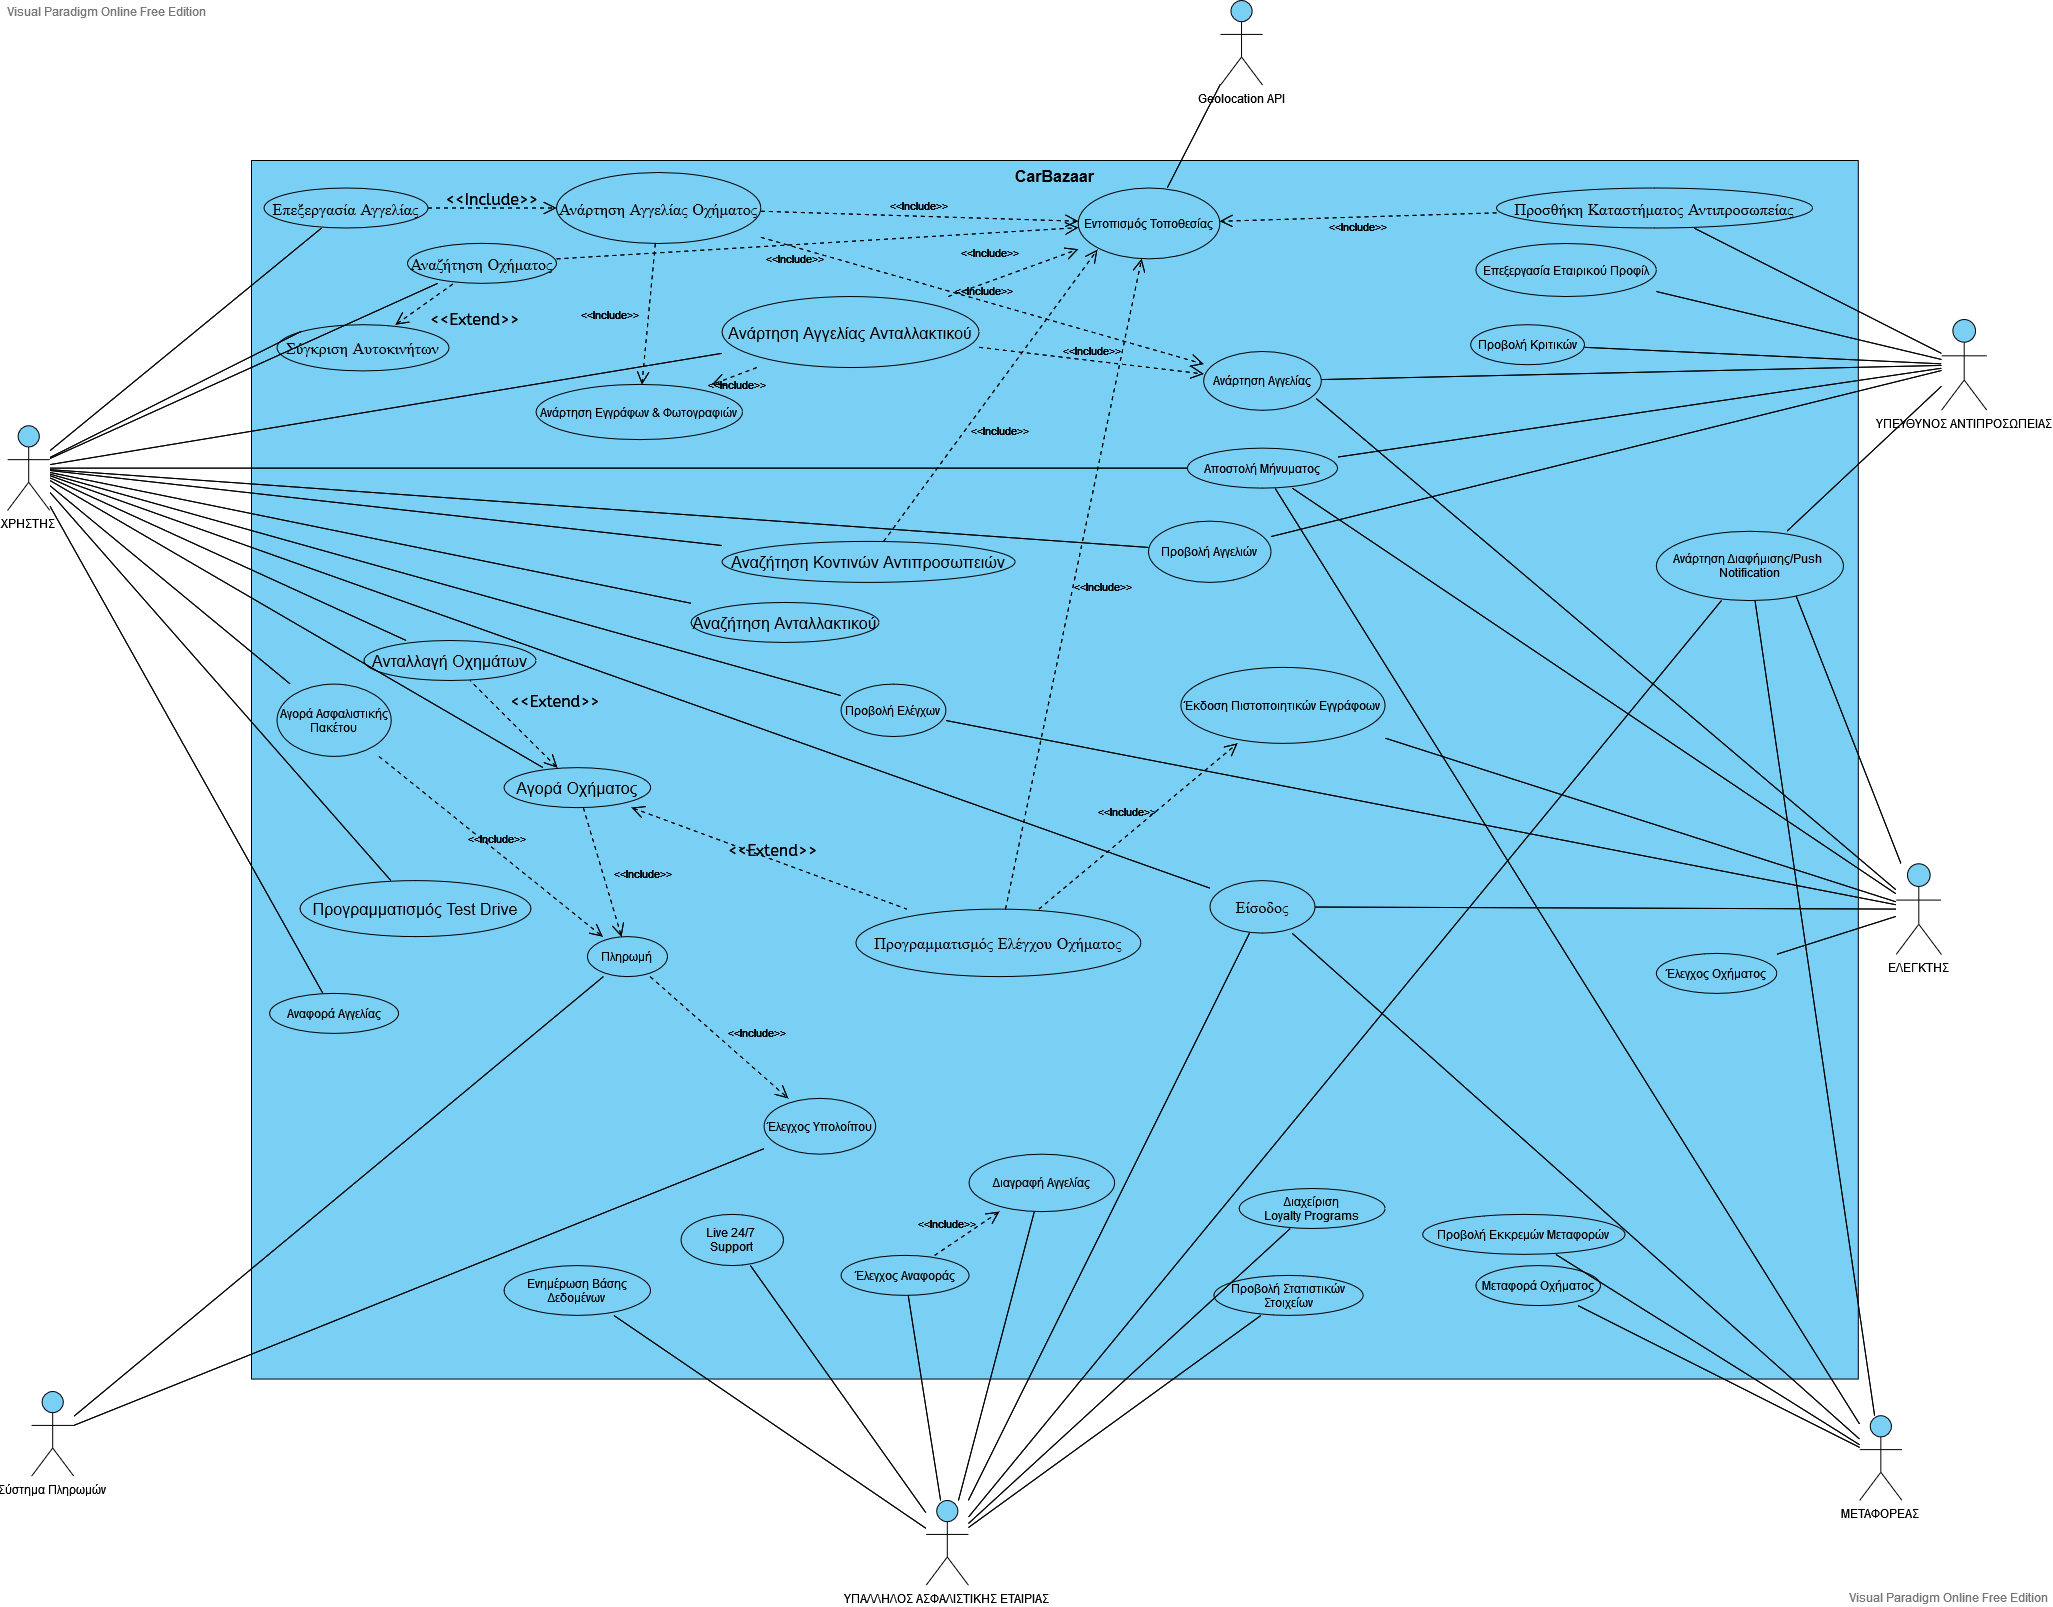
\includegraphics[scale=0.23]{img/UML_Use_case_diagramm.png}
		\caption{\en UML Use Case Diagram \gr}
	\end{figure}
	
	
	
	
\end{document}



